\documentclass{gescons}

\genre {Entrevista}
\author{Luis Claudio Resende}
\title{Da Labilidade Parapsíquica à Assistencialidade Lúcida: Uma Trajetória Evolutiva}

\begin{document}
    \makeentrevistatitle
    \coverart{back/Luis_Claudio_Resende-Labilidade}

    \begin{multicols}{2}


%\noindent\includegraphics[width=9cm, height=10cm]{example-image} 
\begin{center}
    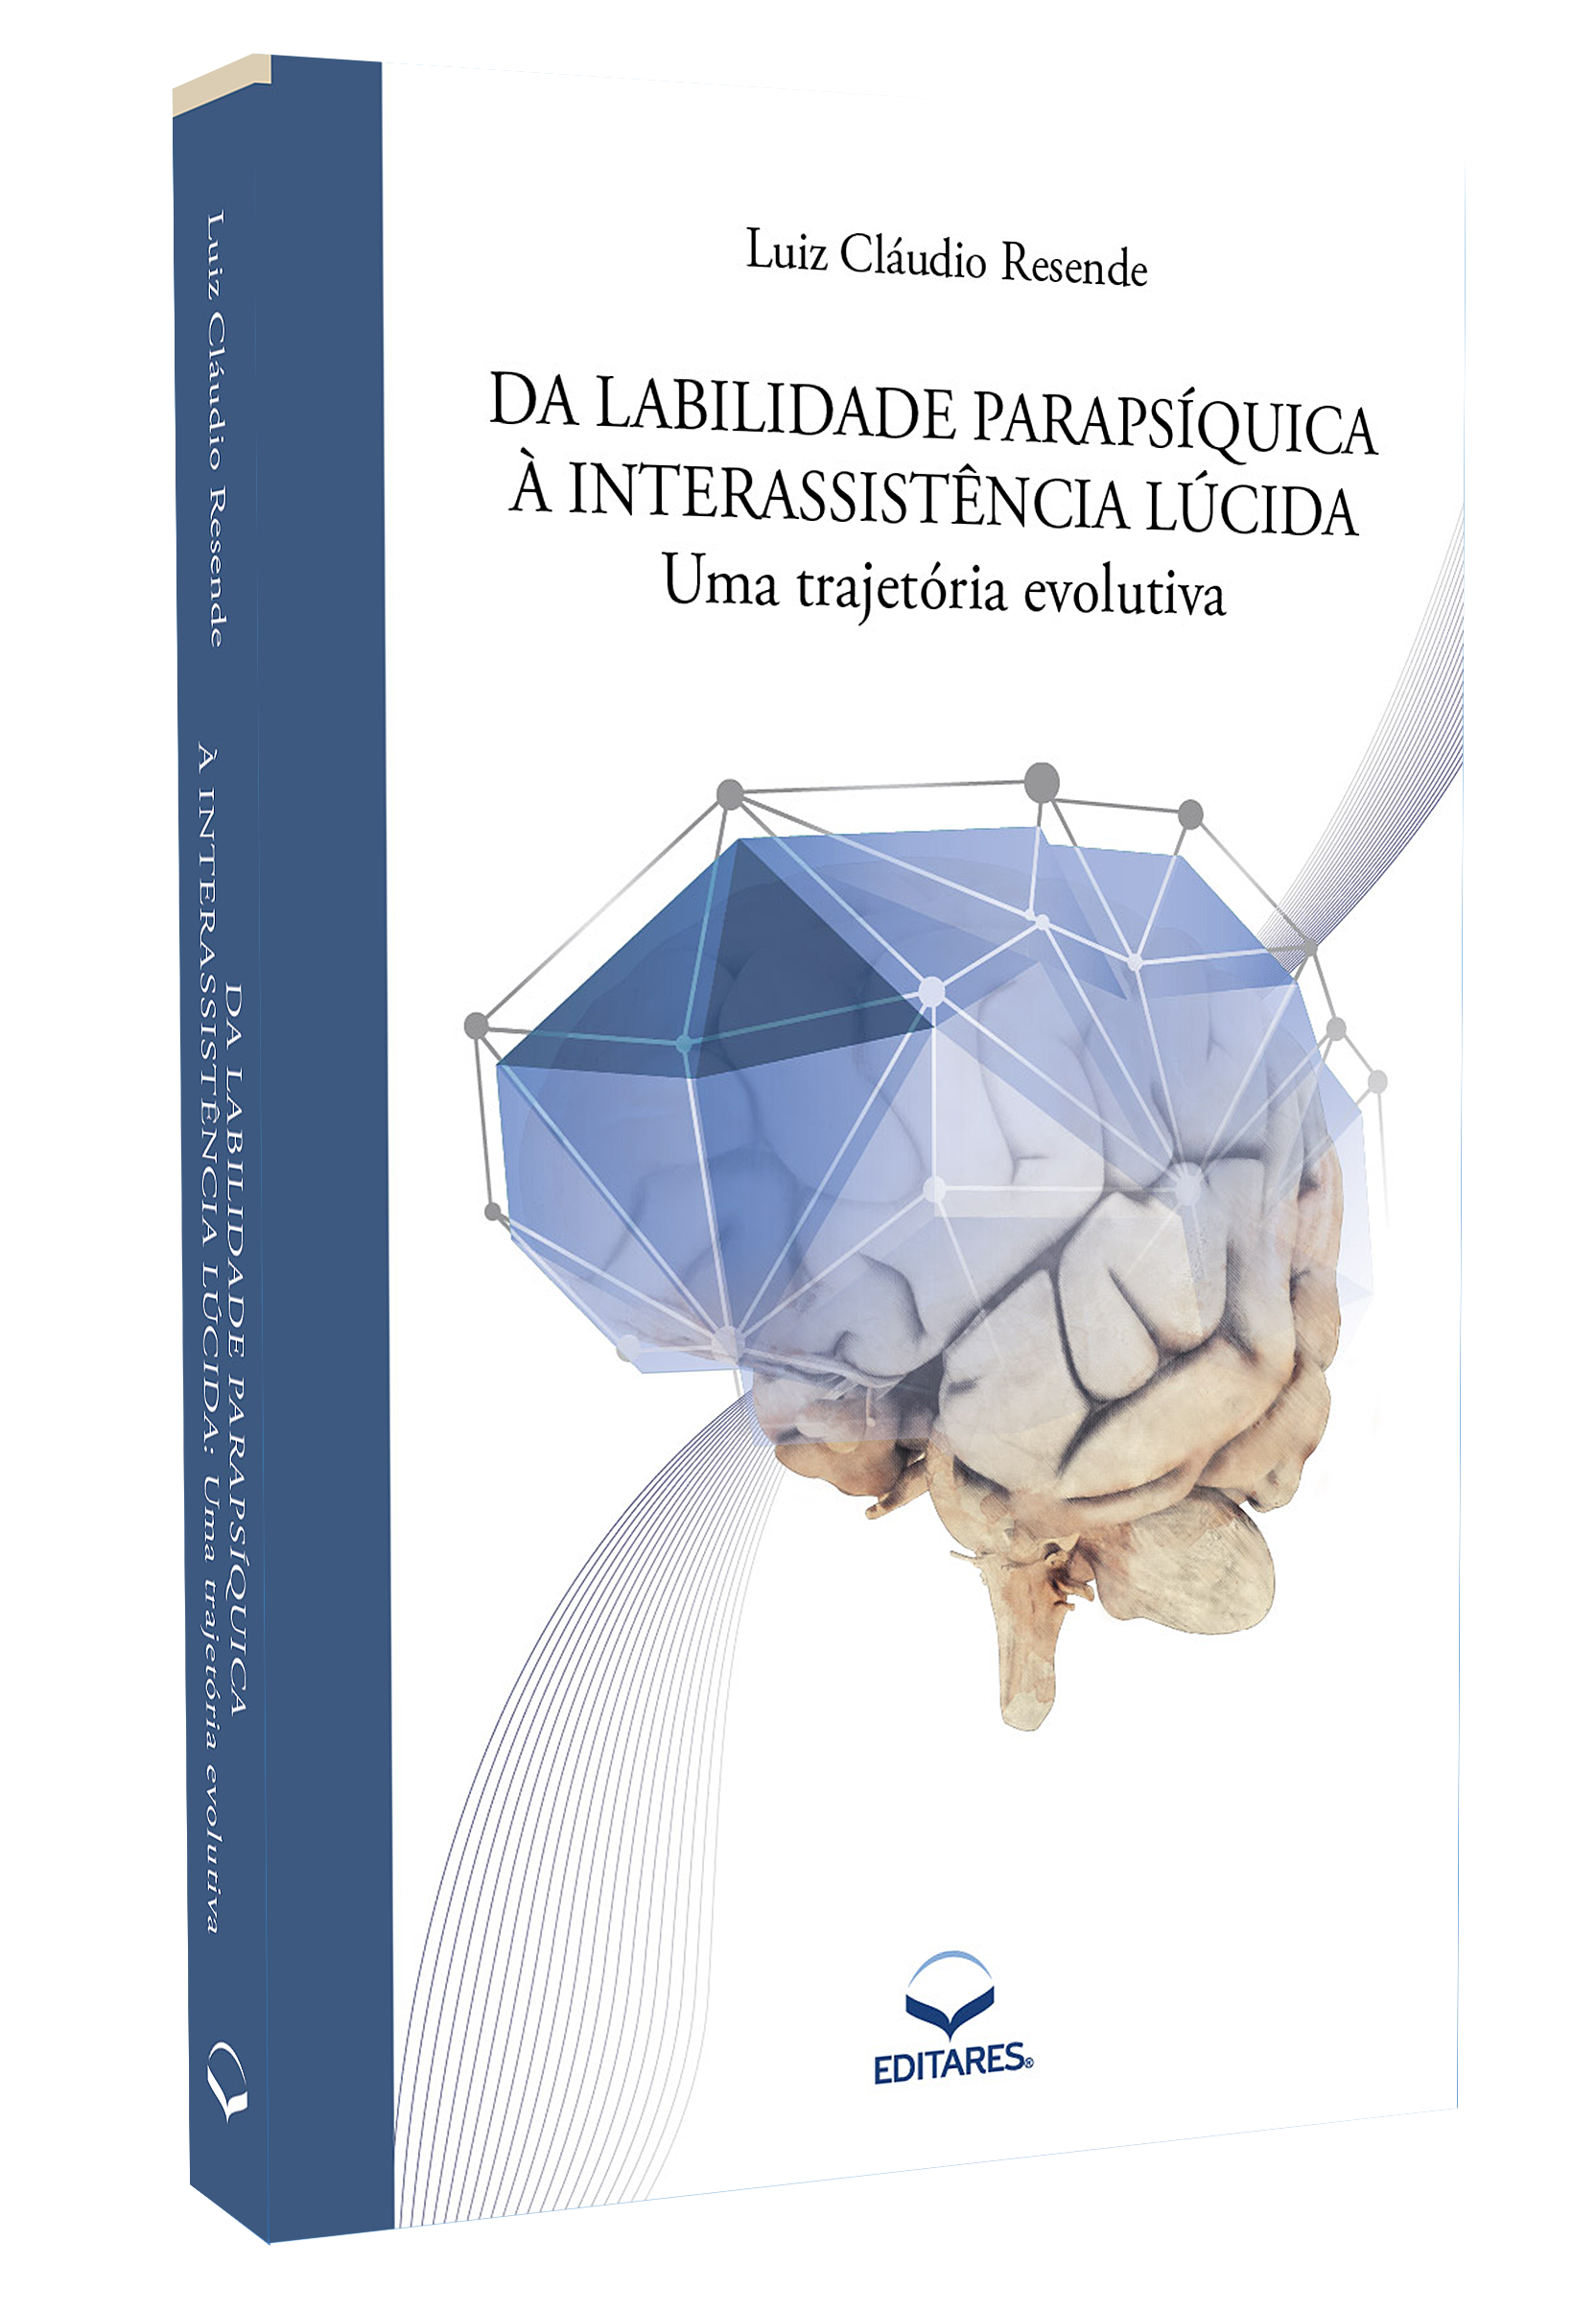
\includegraphics[width=8cm]{articles/entrevista/mockups/Luis_Claudio_Resende-Labilidade.png}
\end{center}

\textbf{1. Qual foi a motivação para a escrita da obra? Por que a definição deste tema para publicação de um livro? }

Após minha última viagem para a França houve a finalização de um ciclo específico de recomposição grupocármica.  Associado a esse fato, havia um conjunto de experiências que poderiam servir de espelho para acelerar processos de resgate e acertos de outras consciências.

O tema principal é a evolução de um quadro de intensa labilidade para maior autocontrole energético e assistencial. 

Como autor e cobaia ao mesmo tempo desse laboratório, optei por escrever algo genuíno e acessível, tendo como público alvo os egressos de cursos intermissivos que tangenciassem a Conscienciologia.  Os relatos das experiências poderiam agir como atratores no processo de recuperação de CONS.

\textbf{2.       Quais foram as principais percepções, intra e extrafísicas, durante a pesquisa e a escrita da obra? E posterior ao lançamento?}

No meu caso específico houve conclusões de autopesquisa e relatos de experiências físicas e multidimensionais. Durante a confecção da obra ocorreu um estado de atividade mentalsomática mais evidente. Ela foi escrita em 60 dias. Optei por escrever da primeira à última página sem  revisar o texto, deixando o fluxo do pensamento mais livre. O resultado final, com ajustes pouco relevantes, deixou-me feliz. Era a minha  história , sob uma ótica mentalsomática, satisfazendo as expectativas iniciais.

\begin{pullquote}
    ``Durante a confecção da obra ocorreu um estado de atividade mentalsomática mais evidente.''
\end{pullquote}


\textbf{3.       Qual o maior aprendizado com a escrita desta obra?}

Foram dois grandes aprendizados:

\begin{itemize}
\item
  A conscin que mais ganha com a obra é aquela que escreve. Ter acesso a uma versão desassediada da sua pensenidade é algo muito interessante. Isso eleva as metas de suas pretensões evolutivas.
\item
  Vivenciando o grau de empenho e trabalho da equipe envolvida na edição, você aprende a valorizar mais o empenho tarístico de todo o grupo
\end{itemize}

\begin{pullquote}
    ``A conscin que mais ganha com a obra é aquela que escreve.''
\end{pullquote}


\textbf{4.       O que poderia dizer como incentivo para que mais pesquisadores invistam na publicação de obras conscienciológicas?}

Apesar dos medos , contrafluxos , repercussões intra e extrafísicas negativas envolvendo uma gescon escrita , vale a pena seguir em frente porque , além de registrar e compartilhar o conhecimento, a obra \emph{per si} chancela suas conquistas evolutivas. 



    


    \end{multicols}
\end{document}


